\documentclass[12pt,a4paper]{article}
\usepackage[utf8]{inputenc}
\usepackage[russian]{babel}
\usepackage{cmap}
%\usepackage{pscyr}
\usepackage{indentfirst}
\usepackage{bm}
\usepackage{amsmath,amssymb}
\usepackage{cite}
\usepackage{color}
\usepackage[colorlinks,urlcolor=blue,citecolor=blue,linkcolor=black,menucolor=black]{hyperref}
\usepackage{graphicx}
\usepackage{epstopdf}
\usepackage{array}
\usepackage{longtable}
\usepackage{amsmath}
\usepackage{amssymb}
\usepackage{amsthm}
\usepackage{amsfonts}
\usepackage{braket}
\usepackage{gensymb}
\usepackage{physics}
\usepackage{listings}
\usepackage{graphicx}
\usepackage{xcolor}
\definecolor{codegreen}{rgb}{0,0.6,0}
\definecolor{codegray}{rgb}{0.5,0.5,0.5}
\definecolor{codepurple}{rgb}{0.58,0,0.82}
\definecolor{backcolour}{rgb}{0.95,0.95,0.92}
\lstdefinestyle{mystyle}{
	backgroundcolor=\color{backcolour}, 
	commentstyle=\color{codegreen},
	keywordstyle=\color{magenta},
	numberstyle=\tiny\color{codegray},
	stringstyle=\color{codepurple},
	basicstyle=\ttfamily\footnotesize,
	breakatwhitespace=false, 
	breaklines=true, 
	captionpos=b, 
	keepspaces=true, 
	numbers=left, 
	numbersep=5pt, 
	showspaces=false, 
	showstringspaces=false,
	showtabs=false, 
	tabsize=2
}
\lstset{
	style=mystyle}

\textwidth 17cm
\textheight 24cm
\oddsidemargin 0cm
\topmargin -1cm

\def\Year{\expandafter\YEAR\the\year}
\def\YEAR#1#2#3#4{#3#4}
\renewcommand{\theequation}{\arabic{section}.\arabic{equation}}
\definecolor{grey}{gray}{0.3}

\begin{document}
	\begin{titlepage}
		\begin{center}
			{\large\bf {Минобрнауки России}\\[12pt]
				Федеральное государственное автономное образовательное \\
				учреждение высшего образования \\
				<<Омский государственный университет им.~Ф.М.~Достоевского>>\\[12pt]
				Физический факультет\\[12pt]
			}
			
			{\large\bf Квазипособие студентам от студентов }\\[12pt]
			{\Large\bf Суперпозиция успеха и отчаяния: Как выжить в мире квантовых вычислений }\\[2cm]
		\end{center}
		\vfill
		\hspace*{7cm}{\bf Составители:}\\[12pt]
		\hspace*{8cm}{\bf  Cтудент  Журавлева Анастасия }\\[12pt]
		\hspace*{8cm}{\bf  Cтудент Коцур Павел }\\[12pt]
		\hspace*{8cm}{\bf  Cтудент  Бахтин Артур}\\[1.5cm]	
		
		\begin{center}
			{\bf Омск -- 2025}
		\end{center}
	\end{titlepage}
	
	\addtocounter{page}{1}
	
	\tableofcontents
	\newpage
	
	\section*{Введение}	
	Настоящие квазипособие представляет собой вводный курс по основам квантовых вычислений, разработанный студенческим коллективом с целью облегчения процесса освоения данного перспективного направления компьютерных наук для учащихся младших курсов. Она также является вводным пособием, разработанным для обеспечения базового понимания квантовых вычислений. Её основная цель – заложить прочный фундамент знаний, необходимый для успешного изучения более сложных материалов, в том числе научных трудов и учебной литературы, предназначенных для продвинутого уровня. Материал данного пособия является результатом анализа и систематизации знаний, полученных авторами в ходе изучения квантовой информатики.\\
	
	Квантовые вычисления, представляющие собой принципиально новый подход к обработке информации, обладают потенциалом для революционного изменения существующих алгоритмов и технологий. Область применения квантовых вычислений охватывает широкий спектр задач, включая, но не ограничиваясь: разработкой новых лекарственных препаратов и материалов, усовершенствование методов искусственного интеллекта, а также развитие криптографических систем.\\
	
	Предлагаемое квазипособие ориентировано на студентов, начинающих знакомство с квантовыми вычислениями. Материал изложен в доступной форме, позволяющей усвоить основные принципы, избегая излишней математической детализации, при этом сохраняя научную корректность. В квазипособии рассматриваются ключевые концепции, такие как квантовые биты (кубиты), принципы суперпозиции и квантовой запутанности, а также базовые квантовые алгоритмы и архитектуры. Основной акцент сделан на предоставлении студентам понимания фундаментальных основ, необходимых для дальнейшего обучения и работы с более сложными источниками информации.\\
	
	Мы надеемся, что это квазипособие станет для вас эффективным средством подготовки к изучению специализированной литературы, облегчит понимание сложных концепций и терминологии, а также позволит вам чувствовать себя увереннее при работе с оригинальными научными публикациями и учебными пособиями по квантовым вычислениям.\\
	
	
	Авторы выражают надежду на вашу успешную работу и желают вам плодотворного обучения.\\
	
	С уважением,\\ Авторы методички\\
	
	\newpage
	\section{Основные положения}
	В данной главе будут рассмотрены основные понятия для квантовых вычислений.
	\subsection{Кубит}
	В классическом понимании информация измеряется битами, которые можно представить как элементарные триггерные системы, принимающие одно из двух двоичных значений: 0 или 1. Биты могут подвергаться изменениям с помощью классических логических операций. В каждый момент времени состояние бита подлежит строгому детерминизму. Однако такая бинарная единица хранения информации не подходит для описания состояния квантовых систем. Поэтому в теории квантовых вычислений вместо классических битов используются кубиты (квантовые биты), для описания состояния которых применяются волновые функции. Таким образом, главное различие между битами и кубитами заключается в том, что кубиты не являются детерминированными и могут находиться в суперпозиции своих логических состояний\cite{1}.
	Как следствие можно записать:\\
	\begin{equation} \label{eq_1}
		\ket{\psi}=\alpha\ket{0}+\beta\ket{1}.
	\end{equation}
	Можно переписать формулу (\ref{eq_1}) как:
	\begin{equation} \label{eq_2}
		\ket{\psi}=e^{i\gamma}\left(\cos(\frac{\theta}{2})\ket{0}+e^{i\phi}\sin(\frac{\theta}{2})\ket{1}\right).
	\end{equation}
	Это уравнение задаёт положение на сфере Блоха. \\
	\begin{figure}[h!]
		\centering
		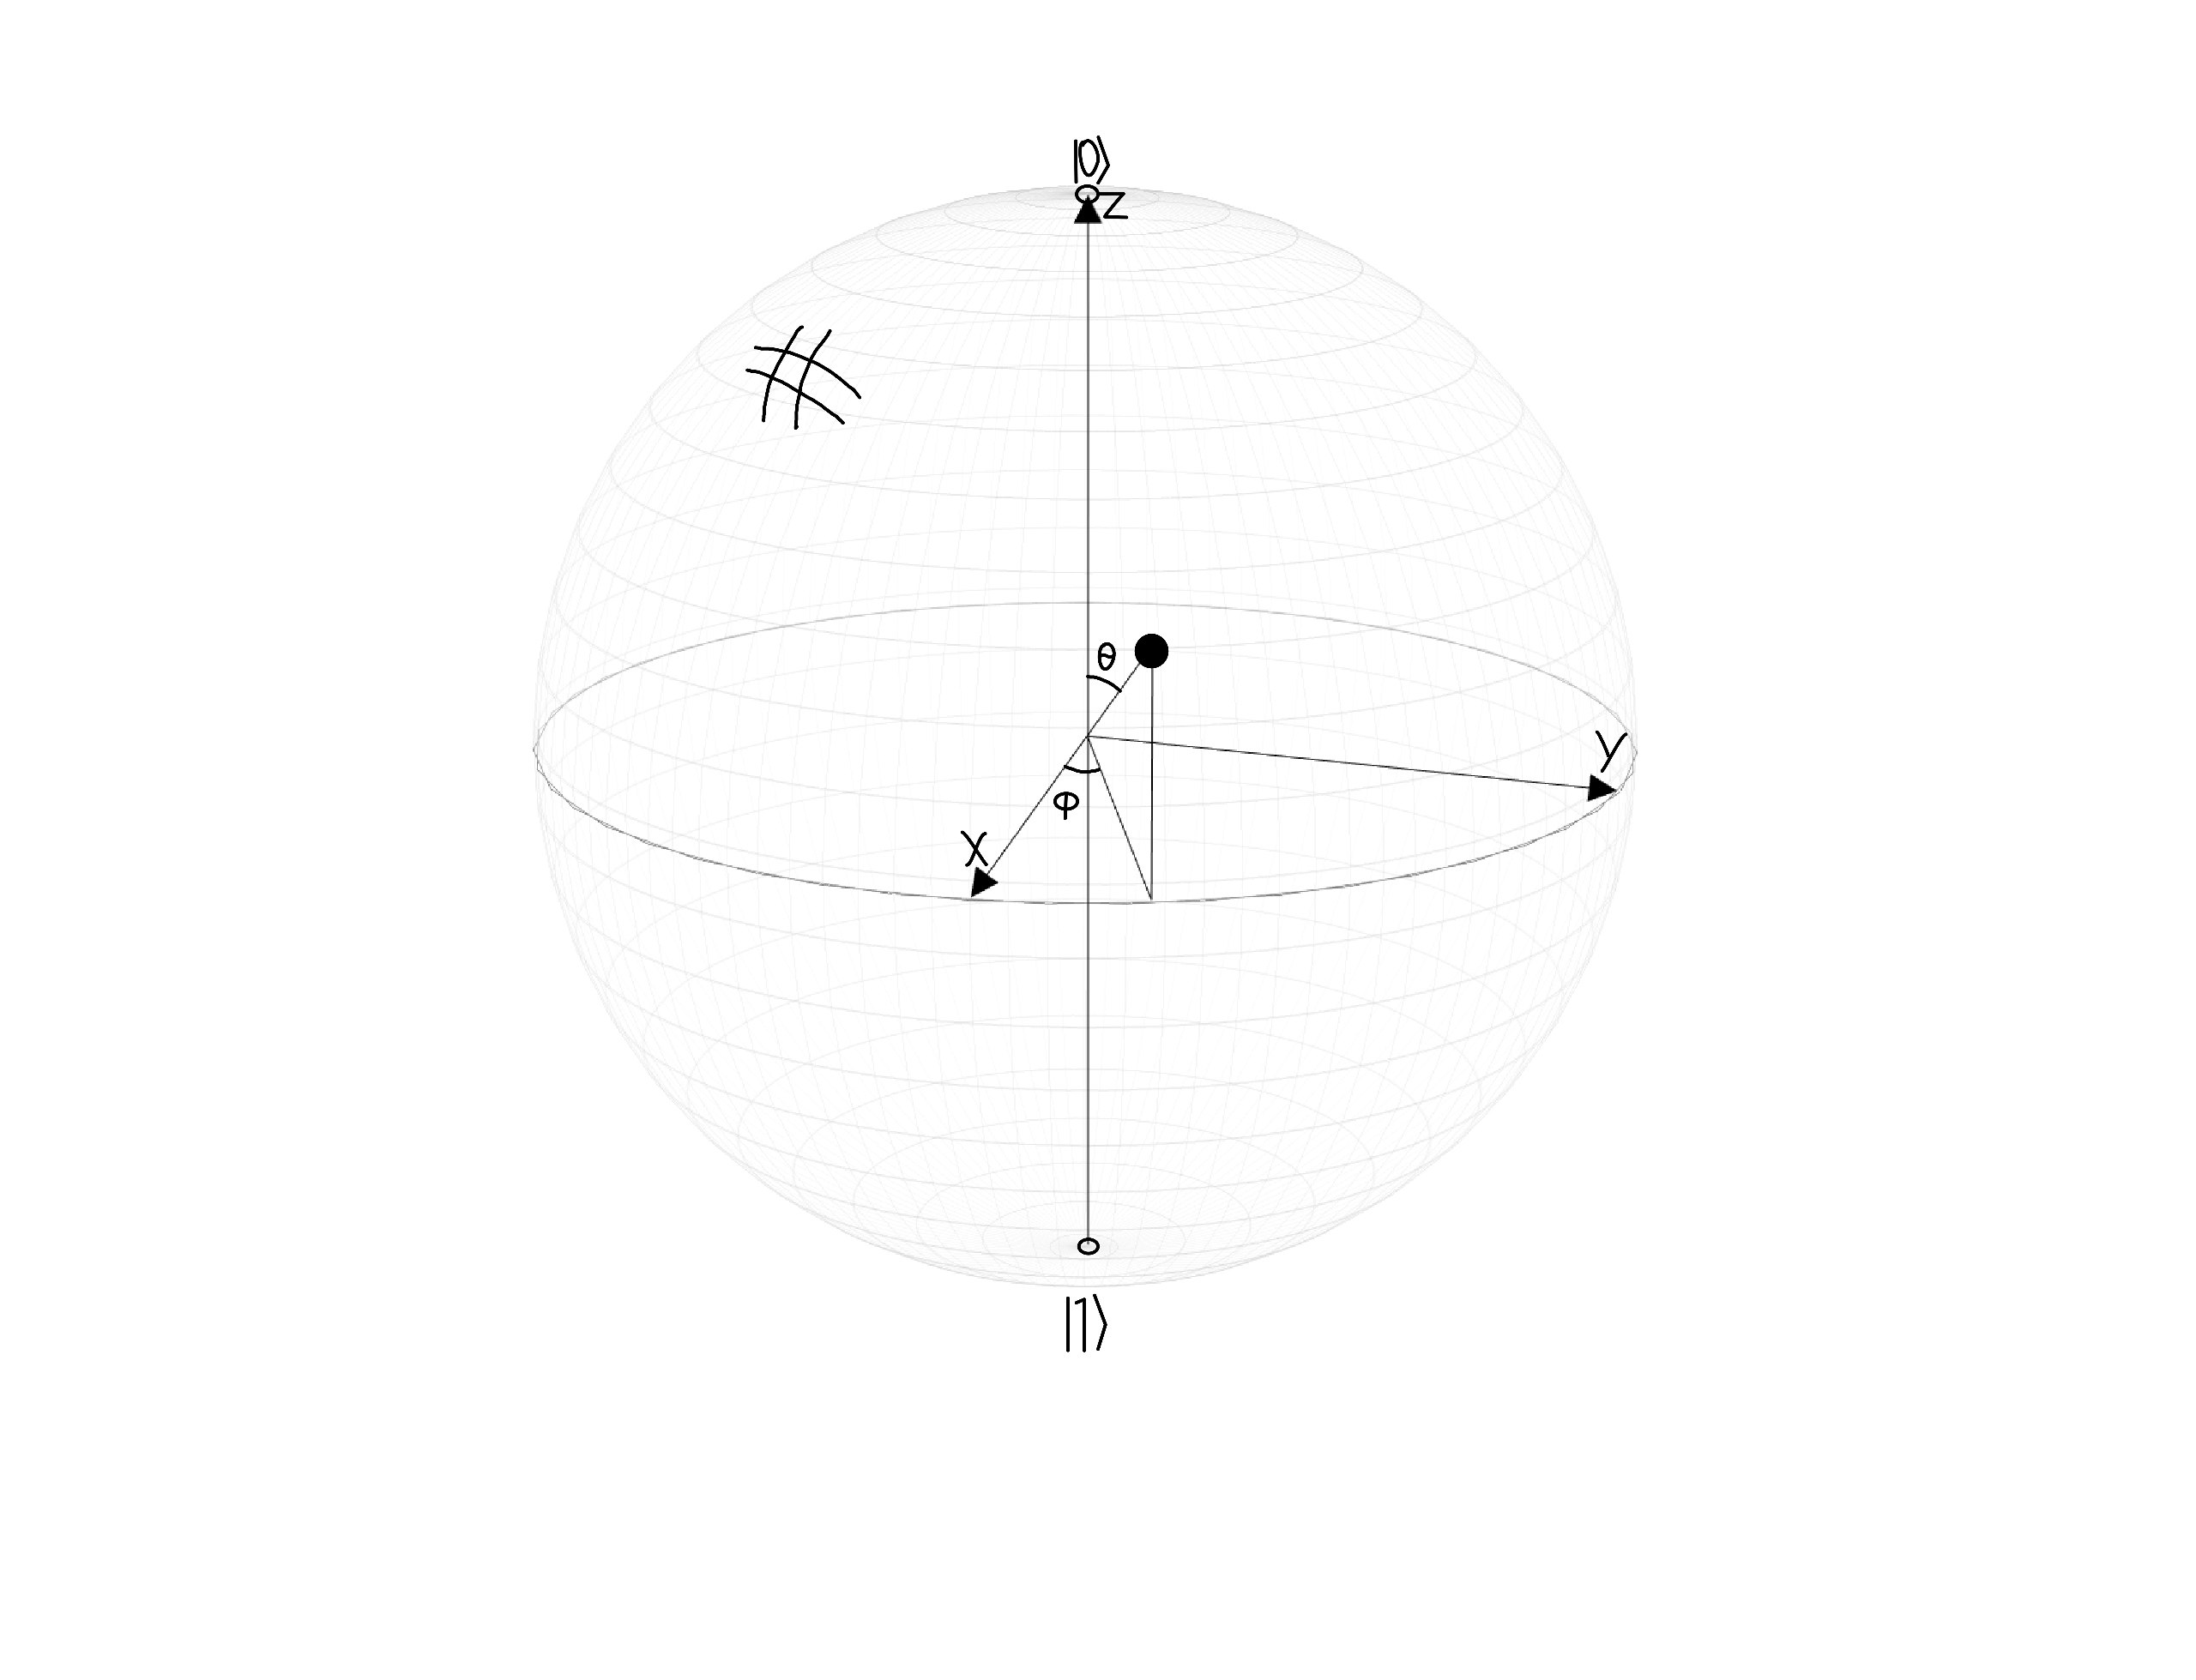
\includegraphics[width=0.7\linewidth]{2.jpg}
		\label{fig_2}\caption{Представление кубита в виде сферы Блоха}
	\end{figure}
	
	В этой сфере континуальное множество точек, как следствие может показаться, что можно закодировать информацию любого объёма. В реальности кубит коллапсирует из суперпозиции в определённое состояние, соответствующее результату измерения.\\
	
	\subsection{Квантовое преобразование Фурье}
	В ортонормированном базисе $\ket{0},...,\ket{N--1}$ квантовое преобразование Фурье определяется как линейный оператор, действующий на базисные состояния по формуле\cite{1}: \\
	\begin{equation}\label{eq_4}
		\ket{j}\longrightarrow\frac{1}{\sqrt{N}}\sum_{k=0}^{N--1}e^{2\pi ijk/N}\ket{k}.
	\end{equation}
	Аналогичным образом действие этого оператора на произвольное состояние можно записать в виде:\\
	\begin{equation}\label{eq_5}
		\sum_{j=0}^{N--1}x_{j}\ket{j}\longrightarrow\sum_{k=0}^{N--1}y_{k}\ket{k},
	\end{equation}
	где амплитуды $y_{k}$ -- дискретные преобразования Фурье амплитуд $x_{j}$. Этот оператор является унитарным, а значит может быть реализован на квантовом компьютере.\par
	Будем считать, что $N=2^{n}$, где $n$ -- целое число, и что базис $\ket{0},...,\ket{2^{n}--1}$ есть вычислительный базис для $n$--кубитового квантового компьютера.\\
	Можно представить квантовое преобразование Фурье в виде произведения:\\
	\begin{equation}\label{eq_6}
		\ket{j_{1},...,j_{n}}\rightarrow\frac{(\ket{0}+e^{2\pi i0.j_{n}}\ket{1})(\ket{0}+e^{2\pi i0.j_{n--1}j_{n}}\ket{1})...(\ket{0}+e^{2\pi i0.j_{1}...j_{n}}\ket{1})}{2^{n/2}}.
	\end{equation}
	Это представление можно считать определением квантового преобразования Фурье. Данное представление
	позволяет построить квантовую схему, эффективно вычисляющую преобразование Фурье, и это доказывает унитарность такого преобразования. Указанное представление позволяет понять алгоритмы, основанные на квантовом преобразовании Фурье. \\
	
	Покажем эквивалентность формулы (\ref{eq_6}) и определения (\ref{eq_4}):\\
	\begin{equation}\label{eq_7}	
		\begin{split} 
			\ket{j}&\rightarrow\frac{1}{2^{n/2}}\sum_{k=0}^{2^{n}--1}e^{2\pi ijk/{2^{n}}}\ket{k}=\\
			&=\frac{1}{2^{n/2}}\sum_{k_{1=0}}^{1}...\sum_{k_{n=0}}^{1}e^{2\pi ij\sum_{l=1}^{n}k_{l}{2^{--l}}}\ket{k_{1}...k_{n}}=\\
			&=\frac{1}{2^{n/2}}\sum_{k_{1=0}}^{1}...\sum_{k_{n=0}}^{1}\bigotimes_{l=1}^{n}e^{2\pi ijk_{l}{2^{--l}}}\ket{k_{l}}=\\
			&=\frac{1}{2^{n/2}}\bigotimes_{l=1}^{n}\left[\sum_{k_{l=0}}^{1}e^{2\pi ijk_{l}{2^{--l}}}\ket{k_{l}}\right]=\\
			&=\frac{1}{2^{n/2}}\bigotimes_{l=1}^{n}\left[\ket{0}+e^{2\pi ij2^{--l}}\ket{1}\right]=\\
			&=\ket{l_{1},...,j_{n}}\rightarrow\frac{(\ket{0}+e^{2\pi i0.j_{n}}\ket{1})(\ket{0}+e^{2\pi i0.j_{n--1}j_{n}}\ket{1})...(\ket{0}+e^{2\pi i0.j_{1}...j_{n}}\ket{1})}{2^{n/2}}.
		\end{split}
	\end{equation}
	Рассмотрим вычисление квантового преобразования Фурье для входного состояния $\ket{j_{1}...j_{n}}$. Для этого введём унитарное преобразование:\\
	\begin{equation}
		R_{k}\equiv\mqty(1&0 \\ 0&e^{2\pi i/2^{k}}).
	\end{equation}
	Применяя элемент Адамара к первому биту, получим состояние:\\
	\begin{equation}
		\frac{1}{2^{1/2}}\left(\ket{0}+e^{2\pi i0.j_{1}}\ket{1}\right)\ket{j_{2}...j_{n}}.	
	\end{equation}
	Поскольку $e^{2\pi i0.j_{1}}$ равно $--1$ при $j_{1}=1$ и $+1$ иначе. Применяя управляемое $R_{2}$, имеем:\\
	\begin{equation}
		\frac{1}{2^{1/2}}\left(\ket{0}+e^{2\pi i0.j_{1}j_{2}}\ket{1}\right)\ket{j_{2}...j_{n}}.
	\end{equation}
	Далее будем применять управляемое $R_{3}$, управляемое $R_{4}$ и т.д. до  $R_{n}$ ( см. п.~\ref{1}), добавляя на каждом шаге по биту к фазе первого из векторов $\ket{1}$. По завершении этой процедуры придем к состоянию:\\
	\begin{equation}
		\frac{1}{2^{1/2}}\left(\ket{0}+e^{2\pi i0.j_{1}j_{2}...j_{n}}\ket{1}\right)\ket{j_{2}...j_{n}}.
	\end{equation}
	Теперь используем ту же процедуру для второго кубита. Элемент Адамара переводит в состояние:\\
	\begin{equation}
		\frac{1}{2^{2/2}}\left(\ket{0}+e^{2\pi i0.j_{1}j_{2}...j_{n}}\ket{1}\right)\left(\ket{0}+e^{2\pi i0.j_{2}}\ket{1}\right)\ket{j_{3}...j_{n}},
	\end{equation}
	Применение управляемых $R_{2},...,R_{n--1}$ даст состояние вида:\\
	\begin{equation}
		\frac{1}{2^{2/2}}\left(\ket{0}+e^{2\pi i0.j_{1}j_{2}...j_{n}}\ket{1}\right)\left(\ket{0}+e^{2\pi i0.j_{2}...j_{n}}\ket{1}\right)\ket{j_{3}...j_{n}},
	\end{equation}
	Продолжая выполнять те же действия для остальных кубитов, придем в конце концов к состоянию:\\
	\begin{equation}
		\frac{1}{2^{2/2}}\left(\ket{0}+e^{2\pi i0.j_{1}j_{2}...j_{n}}\ket{1}\right)\left(\ket{0}+e^{2\pi i0.j_{2}...j_{n}}\ket{1}\right)...\left(\ket{0}+e^{2\pi i0.j_{n}}\ket{1}\right).
	\end{equation}
	Теперь с помощью операции обмена обратим порядок кубитов. После этого получим состояние:\\
	
	\begin{equation}\left(\ket{0}+e^{2\pi i0.j_{n}}\ket{1}\right)
		\frac{1}{2^{2/2}}\left(\ket{0}+e^{2\pi i0.j_{n--1}j_{n}}\ket{1}\right)...\left(\ket{0}+e^{2\pi i0.j_{2}...j_{n}}\ket{1}\right).
	\end{equation}
	
	\section{Ошибки}
	В квантовых вычислениях, подобно классическим, информация подвержена ошибкам. В этой главе мы рассмотрим основные проблемы, связанные с возникновением ошибок в квантовых вычислениях, и почему методы, применяемые в классических вычислениях, здесь не всегда работают. Ключевым препятствием является декогерентизация – взаимодействие квантового компьютера с окружающей средой. Это взаимодействие приводит к потере квантовой информации, подобно тому, как контакт с воздухом разрушает хрупкий предмет.
	\subsection{Основные проблемы}
	
	\subsubsection{Декогерентизация}
	
	Контакт квантового компьютера с окружающей средой (декогерентизация) является основной причиной ошибок, разрушающих квантовую информацию \cite{Preskill}. Представьте себе кубит (квантовый бит) как монету, которая может находиться в состоянии "орла" (\(\ket{0}\)) или "решки" (\(\ket{1}\)), а также в суперпозиции этих состояний (одновременно и орел, и решка). Взаимодействие с внешним миром, например, из-за тепла или электромагнитных помех, может "сбить"\quad  монету, преждевременно определив ее состояние, что эквивалентно потере квантовой информации.
	
	\subsubsection{Неидеальность операций}
	
	Декогерентизация – не единственная проблема. Даже идеальное изолирование от окружающей среды не гарантирует отсутствия ошибок. Представьте себе, что мы хотим применить определенную операцию \(U_0\) к двум кубитам. В реальности эта операция никогда не будет выполнена идеально. Фактическое преобразование будет немного отличаться от запланированного, что можно выразить как небольшую погрешность, порядка \(\epsilon\). Применение операций (квантовых вентилей) многократно, например, около \(\frac{1}{\epsilon}\) раз, приведет к накоплению этих ошибок, что сделает вычисления неточными или даже невозможными.
	
	\subsubsection{Почему классические методы не работают}
	
	Стандартные методы борьбы с ошибками, используемые в классических компьютерах, например, охлаждение, неэффективны в квантовых вычислениях. Охлаждение может повысить точность классической информации, но способно разрушить квантовую информацию, вызвав декогерентизацию. Чтобы сохранить работоспособность квантового компьютера, необходимы методы коррекции ошибок, адаптированные к квантовым особенностям.
	
	\subsection{Специфические трудности коррекции ошибок в квантовых вычислениях}
	
	Квантовая информация более хрупка, чем классическая, и требует специальных методов коррекции ошибок. Рассмотрим основные проблемы:
	
	\subsubsection{Фазовые ошибки}
	
	В дополнение к обычным ошибкам инвертирования битов (\(\ket{0}\rightarrow\ket{1}\) и \(\ket{1}\rightarrow\ket{0}\)), в квантовых вычислениях возникают фазовые ошибки. Эти ошибки изменяют не только значение бита, но и фазу его состояния. Примером фазовой ошибки может быть:
	
	\begin{align}
		\ket{0} &\rightarrow \ket{0} \\
		\ket{1} &\rightarrow --\ket{1}
	\end{align}
	
	Фазовая ошибка особенно опасна, поскольку может перевести состояние в ортогональное ему (математически "противоположное"). Классические методы кодирования, которые хорошо справляются с инверсией битов, не обеспечивают защиты от фазовых ошибок.
	
	\subsubsection{Малые ошибки}
	
	Если кубит находится в суперпозиции:
	
	\begin{equation}
		\alpha\ket{0} + \beta\ket{1},
	\end{equation}
	где \(\alpha\) и \(\beta\) – комплексные числа, описывающие вероятность нахождения кубита в состояниях \(\ket{0}\) и \(\ket{1}\) соответственно, ошибка может изменить значения \(\alpha\) и \(\beta\), пусть и незначительно (на величину порядка \(\epsilon\)). Однако при многократном применении операций эти небольшие ошибки могут накапливаться и в итоге привести к значительным искажениям. Классические же методы коррекции ошибок, как правило, предназначены для исправления больших, а не малых, ошибок.
	
	\subsubsection{Измерение – причина возмущения}
	
	В классических системах для обнаружения и исправления ошибок часто используется принцип голосования (например, если три копии бита, и две из них равны, то считаем значение верным). Для обнаружения и исправления ошибок в квантовых вычислениях требуется измерять кубиты в коде. Однако, измерение кубита в квантовой системе неизбежно возмущает его состояние, то есть разрушает или изменяет информацию, которую он хранит. Это фундаментальное ограничение квантовой механики.
	
	\subsection{Обобщение}
	
	Преодоление проблем, связанных с ошибками в квантовых вычислениях, является одним из самых сложных и важных направлений исследований в этой области. Разработка методов квантовой коррекции ошибок – ключевой шаг на пути к созданию надежных и работоспособных квантовых компьютеров.
	\section{Квантовые вычисления и квантовые компьютеры}
	
	В данной главе будут рассматриваться квантовые вычисления, квантовые алгоритмы, устройство и применение квантовых компьютеров, а также знакомство с синтаксисом языка для квантового компьютера \textit{OPENQASM} 2.0 на примере генератора случайных чисел. 
	%%%%%%%%%%%%%%%%%%%%%%%%%%%%%%%%%%%%%%%%%%%%%%%%%%%%%%%%%%%%%%%%%%%%%%%%%%%%%%%%
	\subsection{Квантовые вычисления. Однокубитовые и многокубитовые гейты. Состояние Белла}
	
	Изменения, происходящие с квантовым состоянием, можно описать на языке квантовых вычислений. Аналогично классическому компьютеру, квантовый компьютер строится из квантовых схем, состоящих из проводов и элементарных квантовых элементов, которые позволяют передавать квантовую информацию и управлять ею. Вычисления реализуют алгоритмически некоторую функцию. Алгоритм имеет множество входных данных и соответствующие им выходные данные.
	
	Любое изменение состояния квантовой системы выражается действием унитарного оператора (гейта). Алгоритм для квантового компьютера представляет собой последовательное применение различных унитарных операторов к некоторому вектору состояния. Оператор $U$ унитарен, если его сопряженный оператор совпадает с обратным:
	\begin{equation}
		UU^{*} = U^{*}U = I,
	\end{equation}
	где $U^{*}$ -- эрмитово сопряженный оператор, $I$ -- единичный оператор. 
	
	\begin{itemize}
		\item \textbf{Оператор Адамара} \\
		Оператор Адамара $H$ является одним из самых полезных квантовых элементов и определяется следующим образом:
		\begin{equation}
			H = H^{*} = \frac{1}{\sqrt{2}}
			\begin{pmatrix}
				1 &  ~~1 \\
				1 & --1
			\end{pmatrix}
		\end{equation}
		Когда оператор Адамара применяется к состоянию кубита, он переводит его в суперпозицию состояний:
		\begin{equation}
			\begin{split}
				& | 0 \rangle \rightarrow \frac{1}{\sqrt{2}}~(| 0 \rangle + | 1 \rangle), \\
				& | 1 \rangle \rightarrow \frac{1}{\sqrt{2}}~(| 0 \rangle-- | 1 \rangle).
			\end{split}
		\end{equation}
		\item \textbf{Гейт $X$} \\
		Гейт $X$ -- квантовый аналог классического вентиля $NOT$.
		\begin{equation}
			X = 
			\begin{pmatrix}
				0 & 1 \\
				1 & 0
			\end{pmatrix},
		\end{equation}
		Применим гейт $X$ к состояниям $|0 \rangle$ и $|1 \rangle$:
		\begin{equation}
			X |0 \rangle = 
			\begin{pmatrix}
				0 & 1 \\
				1 & 0
			\end{pmatrix}
			\begin{pmatrix}
				1 \\
				0
			\end{pmatrix}
			=
			\begin{pmatrix}
				0 \\
				1
			\end{pmatrix}
			=  |1 \rangle,
		\end{equation}
		
		\begin{equation}
			X |1 \rangle = 
			\begin{pmatrix}
				0 & 1 \\
				1 & 0
			\end{pmatrix}
			\begin{pmatrix}
				0 \\
				1
			\end{pmatrix}
			=
			\begin{pmatrix}
				1 \\
				0
			\end{pmatrix}
			=  |0 \rangle.
		\end{equation}
		
		\item \textbf{Гейт $CNOT$} \\
		Гейт $CNOT$ применяется для системы из двух кубитов, и
		предназначен для четырехмерного пространства:
		\begin{equation}
			CNOT = 
			\begin{pmatrix}
				1 & 0 & 0 & 0 \\
				0 & 1 & 0 & 0 \\
				0 & 0 & 0 & 1 \\
				0 & 0 & 1 & 0 
			\end{pmatrix}.
		\end{equation}
		Гейт $CNOT$ действует как условный $NOT$, а именно если первый кубит (управляющий) равняется единице, то на второй (управляемый) действует гейт $NOT$. Если первый равняется нулю, то на второй ничего не действует. Базис после применения данного гейта выглядит следующим образом:
		\begin{equation}
			\begin{split}
				&CNOT~|00\rangle = |00\rangle, \\
				&CNOT~|01\rangle = |01\rangle, \\	
				&CNOT~|10\rangle = |11\rangle, \\
				&CNOT~|11\rangle = |10\rangle.
			\end{split}
		\end{equation}
	\end{itemize}
	Рассмотрим ситуацию, в которой содержится гейт Адамара с последующим применением гейта $CNOT$. Сначала преобразование Адамара переводит верхний кубит в состояние суперпозиции, затем эта суперпозиция поступает на управляющий вход $CNOT$, и управляемый кубит меняет значение, если значение управляющего кубита равно 1. Полученные выходные состояния называются состояниями Белла, или ЭПР -- состояниями, в честь тех людей, которые первыми указали на странные свойства подобных состояний -- Белла, Эйнштейна, Подольского, Розена~\cite{1}:
	\begin{equation}
		\begin{split}
			&|\beta_{00} \rangle = \frac{|00 \rangle + |11\rangle}{\sqrt{2}}, \\
			&|\beta_{01} \rangle = \frac{|01 \rangle + |10\rangle}{\sqrt{2}}, \\
			&|\beta_{10} \rangle = \frac{|00 \rangle -- |11\rangle}{\sqrt{2}}, \\
			&|\beta_{11} \rangle = \frac{|01 \rangle -- |10\rangle}{\sqrt{2}}.
		\end{split}
	\end{equation}
	Состояния Белла демонстрируют квантовую запутанность. Если две частицы находятся в состоянии Белла, их состояния нельзя описать независимо. Измерение одной частицы мгновенно определяет состояние другой, даже если они находятся на огромном расстоянии (ЭПР--парадокс).
	%%%%%%%%%%%%%%%%%%%%%%%%%%%%%%%%%%%%%%%%%%%%%%%%%%%%%%%%%%%%%%%%%%%%%%%%%%%%%%%%
	\subsection{Квантовый язык программирования \textit{OPENQASM} 2.0. Генератор случайных чисел на квантовом компьютере}
	Квантовые языки программирования предназначены для описания квантовых алгоритмов, моделирования квантовых схем и взаимодействия с реальными квантовыми компьютерами. Язык \textit{OPENQASM (Quantum Assembly Language)} 2.0~\cite{openqasm} служит для описания квантовых алгоритмов в императивном стиле. Это один из ключевых низкоуровневых  языков, используемых в квантовых вычислениях. Он используется в квантовых фреймворках (например, $Qiskit$ преобразует $Python$--код в \textit{OPENQASM} 2.0 перед отправкой на квантовый компьютер), квантовых симуляторах \textit{IBM Quantum Lab}, эмуляторе квантового компьютера <<Телеквант>>~\cite{Telequant}.
	
	Программа начинается со строки \textit{OPENQASM} 2.0, далее следует объявление квантовых и классических переменных которые будут использоваться как ячейки хранения информации. После объявления переменных следует тело программы, в котором к квантовым переменным применяются квантовые операции и квантовые измерения с последующей записью результата измерения в классическую переменную. Квантовый регистр используется для генерации случайного бита, а классический -- для хранения результата измерения. По завершению программы результатом ее работы являются данные, записанные в классические переменные. Состояния квантовых переменных не доступны для пользователя в силу фундаментальных принципов квантовой механики. Извлечь информацию из квантовых переменных можно только средствами квантовых измерений. Все объявленные классические переменные инициализируются $0$, все объявленные квантовые переменные инициализируются состоянием |0$\rangle$. Время жизни всех квантовых и классических переменных совпадает со временем жизни программы~\cite{Telequant}.
	Как пример рассмотрим генератор случайных чисел, написанный на языке \textit{OPENQASM} 2.0 для эмулятора квантового компьютера <<Телеквант>>~\cite{Telequant}. В рамках реализации генератора случайных чисел для 10 кубитов используется следующий алгоритм:
	\begin{enumerate}
		\item Инициализация \\
		Создается квантовый регистр q[10] из 10 кубитов и классический регистр c[10] для хранения результатов измерений.
		\item Применение гейта Адамара \\
		После преобразования Адамара состояния кубитов распределятся с равной вероятностью.
		\item Измерение состояния кубитов \\
		На этом этапе производится измерение состояния кубитов с сохранением результатов. Полученные значения интерпретируются как случайные биты.
	\end{enumerate}
	Программный код для измерения 10 кубитов: \\\\
	\texttt{OPENQASM 2.0;\\
		include "qelib1.inc";\\
		qreg q[10];\\
		creg c[10];\\
		h q[0];\\
		\vdots \\
		h q[9];\\
		measure q[0] $\rightarrow$ c[0];\\
		\vdots \\
		measure q[9] $\rightarrow$ c[9];\\}
	
	Программа начинается со строки \textit{OPENQASM} 2.0, где 2.0 -- используемая версия языка.
	Далее подключается стандартная библиотека квантовых операций, включающая в себя необходимый для генерации случайных чисел гейт Адамара $h$. Далее объявляется квантовый qreg и классический creg регистры. Квантовый регистр используется для генерации случайного бита, а классический -- для хранения результата измерения. После следует применения гейта Адамара $h$, который переводит кубит из состояния $\ket{0}$ в суперпозицию. Это означает, что при измерении кубит с равной вероятностью окажется в состоянии  $\ket{0}$ или  $\ket{1}$.
	Все объявленные классические переменные инициализируются нулем, все объявленные квантовые переменные инициализируются состоянием |0$\rangle$. Последняя строка измеряет кубит $q[0]$ и сохраняет результат в классический бит $c[0]$. Результат измерения будет случайным: $0 $ или $1$.	
	
	\subsection{Квантовый компьютер}
	
	Основной интерес к теории квантовых вычислений и квантовой информации связан с тем, что необходимые для обработки алгоритмов устройства действительно могут быть реализованы, а не просто являются математическими моделями. Экспериментальная реализация квантовых схем является очень сложным процессом, в котором должны обязательно одновременно выполняться несколько принципов: чтобы сохранять квантовые состояния, квантовый компьютер должен быть хорошо изолирован от окружающей среды, и его кубиты должны быть достаточно доступны, чтобы можно было выполнять вычисления и считывать результаты~\cite{1}. Трудности в реализации связаны с тем, что чаще всего можно удовлетворить только часть требований. Например, монета является хорошим представлением бита, но плохим представлением кубита, поскольку находится в суперпозиции очень короткое время. При оценке качества  и перспективности системы ключевую роль играет понятие квантового шума.
	
	\section{Квантовая информация}
	В этой главе мы погрузимся в основы квантовой информации, изучая ключевые концепции и их удивительные приложения. Во многом затронутые темы будут носить фундаментальный характер. Настоятельно рекомендуется перевести дух и только после этого окунуться в изучение квантовой информации с новыми силами и зарядом бодрости.
	\subsection{Квантовая информация в квантовых каналах}
	В области квантовых вычислений распространены два разных значения для термина квантовая информация. Во--первых, он применяется в качестве общего названия для всех видов деятельности, связанных с обработкой информации на основе квантовой механики. Во втором значении этот термин более специализирован: он относится к изучению элементарных задач по обработке квантовой информации\cite{1}.\\
	\indent В классической теории информации доказываются теоремы Шеннона о кодировании применительно к сжатию и развертыванию квантовых состояний. Рассмотрим различные квантовые аналоги этих теорем. Для начала выберем за квантовый источник информации квантовые состояния $\ket{\psi_{j}}$, описываемые набором вероятности $p_{j}$. Таким образом каждое обращение независимо и даёт с вероятностью $p_{j}$ состояние  $\ket{\psi_{j}}$. Здесь возникает двоякая ситуация. К примеру мы имеем состояния $\ket{0}$ и $\ket{1}$, описываемые вероятностями $p$ и $1--p$, соответственно, тогда можно применить теорему Шеннона точно так же как и для классического случая. Мы получим что необходимое число кубитов будет $H(p,1--p)$, где $H$ -- энтропия Шеннона. ($H(p_{j})=--\sum_{j}p_{j}\log(p_{j})$). Но если мы будем иметь в каком--то из случаев, допустим, состояние Белла, использовать классический подход в лоб нельзя, так как мы не различаем состояния Белла и, условно,  $\ket{0}$. \\
	\indent Даже в этом случае можно произвести сжатие, только оно перестаёт быть безошибочным в том смысле, что квантовые состояния на выходе источника могут слегка искажаться процедурой сжатия--развертывания. Чтобы охарактеризовать искажения вводят понятие совпадения (fidelity), которое определяет среднее искажение, вносимое этим алгоритмом. Идея состоит в том, что сжатые данные должны восстанавливаться с очень большой точностью.\\
	\indent Теорема Шумахера о кодировании для канала без шума устанавливает, какое количество ресурсов требуется для сжатия квантовых данных при условии, что источник можно восстановить с точностью близкой к 1, что означает отсутствие ошибок. Теорема в нашем определении источника информации сводится к утверждению о том, что возможно сжатие не более, чем до классического предела $H(p_{j})$. Здесь кроется одна деталь -- это верно для ортогональных  $\ket{\psi_{j}}$. В общем случае надо вводить энтропию фон Неймана, которая совпадает с энтропией Шеннона только в случае ортогональности. В противном случае энтропия фон Неймана строго меньше энтропии Шеннона. Так для примера с состоянием Белла и $\ket{0}$ понадобится меньше число кубитов, чем  $H(p,1--p)$.
	\subsection{Квантовая различимость}
	В квантовомеханическом случае не всегда можно различить произвольные состояния, например возникает неразличимость  неортогональных квантовых состояний. Тем самым квантовое состояние содержит скрытую информацию, недоступную для измерения. Неразличимость на <<пальцах>> доказывается от обратного, если бы мы могли точно различить состояния неортогональной системы, то передача информации была бы больше скорости света, что невозможно по физическим причинам\cite{1}.		
	\subsection{Квантовый параллелизм}
	
	Квантовый параллелизм -- это фундаментальное свойство квантовых вычислений, позволяющее выполнять вычисления над всеми возможными входными данными одновременно. В отличие от классических компьютеров, которые обрабатывают данные последовательно, квантовые компьютеры используют суперпозицию квантовых битов (кубитов), чтобы находиться во всех возможных состояниях одновременно. Это позволяет квантовому алгоритму одновременно исследовать все возможные решения задачи, что значительно ускоряет вычисления для определенного класса задач. Однако, важно отметить, что квантовый параллелизм не означает мгновенного получения всех результатов; информация о всех возможных исходах содержится в суперпозиции, и извлечение нужного результата требует процесса измерения, который разрушает суперпозицию. Тем не менее, эта одновременная обработка информации является ключевым фактором, обеспечивающим превосходство квантовых компьютеров над классическими в решении определенных типов задач.
	\subsection{Плотное кодирование}
	Плотное кодирование использует зацепленные состояния Белла, например, $|\Phi^+\rangle = \frac{1}{\sqrt{2}}(|00\rangle + |11\rangle)$. Алиса, имеющая один кубит из зацепленной пары, применяет к нему один из четырех унитарных операторов $\{I, \sigma_x, \sigma_z, \sigma_x \sigma_z\}$, где $I$ -- единичный оператор, $\sigma_x$ -- оператор Паули $X$, $\sigma_z$ -- оператор Паули $Z$. Каждый оператор соответствует одному из четырех возможных двухбитных состояний $(00, 01, 10, 11)$. Затем Алиса отправляет свой кубит Бобу. Боб, выполнив совместное измерение на своей и полученной от Алисы паре кубитов в базисе Белла, определяет, какой оператор был применен Алисой, восстанавливая таким образом два классических бита информации.
	\subsection{Квантовая телепортация}
	Квантовая телепортация -- это процесс передачи квантового состояния от одного кубита (отправителя) к другому (получателя) с использованием зацепленных частиц и классической связи. Важно отметить, что сама *материя* не перемещается, а лишь квантовое состояние.
	
	\subsubsection{Схема телепортации}
	
	Для телепортации требуется:
	
	\begin{itemize}
		\item \textbf{Отправитель (Алиса)}: Кубит в неизвестном состоянии $\ket{\psi} = \alpha \ket{0} + \beta \ket{1}$, где $\alpha$ и $\beta$ -- комплексные амплитуды.
		\item \textbf{Получатель (Боб)}: Кубит в известном состоянии, например, $\ket{0}$.
		\item \textbf{Зацепленная пара кубитов}: Пара зацепленных кубитов, по одному у Алисы и Боба, в состоянии Белла $\ket{\Phi^+} = \frac{1}{\sqrt{2}}(\ket{00} + \ket{11})$.
	\end{itemize}
	
	
	\subsubsection{Процесс}
	
	1. \textbf{Совместное измерение}: Алиса выполняет совместное измерение своего кубита $\ket{\psi}$ и своего кубита из зацепленной пары в базисе Белла. Результат измерения может быть одним из четырех состояний Белла: $\ket{\Phi^+}$, $\ket{\Phi^--}$, $\ket{\Psi^+}$, $\ket{\Psi^--}$.
	
	2. \textbf{Классическая коммуникация}: Алиса передает результаты своего измерения (два классических бита) Бобу по классическому каналу связи.
	
	3. \textbf{Восстановление состояния}: В зависимости от полученных от Алисы битов, Боб выполняет соответствующую унитарную операцию над своим кубитом из зацепленной пары. Это восстанавливает исходное состояние $\ket{\psi}$ на кубите Боба.
	
	\subsubsection{Математическое описание}
	
	Состояние всей системы до измерения:\\
	\begin{equation}
		\ket{\psi} \otimes\ket{\phi^{+}}=(\alpha\ket{0} + \beta \ket{1})\otimes \frac{1}{\sqrt{\ket{00} +\ket{11}}}
	\end{equation}
	В зависимости от результатов измерения Алисы, Боб применяет следующие операции:
	\begin{itemize}
		\item $\ket{\Phi^{+}}$: $I$ (единичный оператор)
		\item $\ket{\Phi^{--}}$: $\sigma_{z}$ (оператор Паули Z)
		\item $\ket{\Psi^{+}}$: $\sigma_{x}$ (оператор Паули X)
		\item $\ket{\Psi^{--}}$: $\sigma_{x} \sigma_{z}$
	\end{itemize}
	\subsection{Квантовая криптография}
	\subsubsection{Распределение квантового ЭПР--ключа}
	У каждого есть секреты. Боб и Алиса хотят передать информацию в совершенном секрете, проблема в том, что их подруга Ева хочет всё подслушать. Предположим Боб и Алиса не способны придумать классический шифр, который не взломала бы Ева. Есть единственный способ передать биты так, чтобы Ева их не узнала, но предположим Алиса и Боб хотят установить общий случайный ключ. Можно использовать протоколы открытых ключей, но Ева и здесь перехитрила наших героев, она обладает невероятно сильной вычислительной машиной. Но Боб и Алиса будут использовать квантовые ключи, тем самым смогут защититься от посягательств от Евы. \\
	\indent Предположим, что Алиса и Боб делят запас запутанных пар, приготовленных в состоянии $\ket{\phi^{+}}$. Чтобы приготовить известный только им ключ необходимо выполнить следующий протокол.\\
	\indent Для каждого кубита они измеряют $\sigma_{1}$ или $\sigma_{3}$. Это решение псевдослучайное. Затем они открыто объявляют о том, какие наблюдаемые были измерены, но не открывают полученные ими результаты. Кубиты, измеренные вдоль разных осей, получаются нескоррелированные, их отбрасывают. В тех случаях, где измерения выполнены вдоль одних и тех же осей, их результаты хотя и случайны, но идеально скоррелированны. Ева не может, измеряя свои кубиты, вычислить код. Чтобы убедиться в том, что их состояния скоррелированы, Алиса и Боб открывают часть ключа и сверяются. Если Ева попытается вмешаться в передачу, то Боб и Алиса выбросят ключи и создадут новый. Конечно же можно предположить ещё варианты. В реальности будут возникать помехи, которые можно устранить разными способами.
	\subsection{Невозможность клонирования} 
	В классической физике копирование информации -- тривиальная задача. Однако в квантовой механике это невозможно из-за принципа суперпозиции и теоремы о запрете клонирования. Эта теорема утверждает, что невозможно создать точную копию произвольного неизвестного квантового состояния. Попытка клонирования неизбежно приведет к нарушению принципов квантовой механики.
	
	\subsubsection{Формулировка теоремы}
	
	Рассмотрим два кубита: исходный кубит в неизвестном состоянии $\ket{\psi} = \alpha\ket{0} + \beta\ket{1}$ и вспомогательный кубит, который изначально находится в известном состоянии $\ket{0}$. Цель -- создать устройство (квантовый клоннер), которое преобразует состояние $\ket{\psi} \otimes \ket{0}$ в состояние $\ket{\psi} \otimes \ket{\psi}$.
	
	Предположим, существует унитарный оператор $U$, который выполняет клонирование:
	\begin{equation}
		U (\ket{\psi} \otimes \ket{0}) = \ket{\psi} \otimes \ket{\psi}
	\end{equation}
	Для доказательства невозможности клонирования воспользуемся методом от противного. Предположим, что такой оператор $U$ существует. Рассмотрим два разных состояния: $\ket{\psi_1} = \alpha_1\ket{0} + \beta_1\ket{1}$ и $\ket{\psi_2} = \alpha_2\ket{0} + \beta_2\ket{1}$. Если клонирование возможно, то:
	\begin{equation}
		U (\ket{\psi_1}  \otimes \ket{0}) = \ket{\psi_1}  \otimes  \ket{\psi_1}
	\end{equation}
	\begin{equation}
		U (\ket{\psi_2}  \otimes \ket{0}) = \ket{\psi_2} \otimes  \ket{\psi_2}
	\end{equation}
	Теперь вычислим скалярное произведение этих двух состояний:
	\begin{equation}
		\braket{\psi_1 \otimes \psi_1}{\psi_2 \otimes \psi_2}=(\braket{\psi_1}{\psi_2})^{2}
	\end{equation}
	С другой стороны, поскольку $U$ -- унитарный оператор, он сохраняет скалярное произведение:
	\begin{equation}
		\braket{\psi_1 \otimes \psi_1}{\psi_2 \otimes \psi_2}=	\bra{\psi_1 \otimes 0}U^\dag U \ket{\psi_2 \otimes 0}=\braket{\psi_1}{\psi_2}
	\end{equation}
	Из этих двух уравнений следует:
	\begin{equation}
		(\braket{\psi_1}{\psi_2})=(\braket{\psi_1}{\psi_2})^{2}
	\end{equation}
	
	Это уравнение выполняется только в двух случаях: $\langle \psi_1 | \psi_2 \rangle = 0$ или $\langle \psi_1 | \psi_2 \rangle = 1$. Это означает, что состояния $\ket{\psi_1}$ и $\ket{\psi_2}$ либо ортогональны, либо идентичны. Однако это противоречит тому, что $\ket{\psi_1}$ и $\ket{\psi_2}$ -- произвольные состояния. Следовательно, наше предположение о существовании унитарного оператора $U$ неверно.
	
	
	\section{Практическая реализация}
	Это заключительная глава, направленная на практическую часть. Ниже представлен программный код на языке Python, использующий библиотеку Qiskit, который демонстрирует построение и применение (в данном случае, обратного) квантового преобразования Фурье. После ознакомления с примером кода будет дано подробное пояснение используемых компонентов Qiskit, а также базовых концепций языка Python, необходимых для понимания представленной реализации.
	
	\subsection{Квантовое преобразование Фурье}
	Программа:
	\begin{lstlisting}[language=Python]
		from qiskit import QuantumCircuit,transpile
		from qiskit.quantum_info import Kraus, SuperOp
		from qiskit.visualization import plot_histogram
		from qiskit.transpiler.preset_passmanagers import generate_preset_pass_manager
		from qiskit_aer import Aer
		from qiskit.visualization import plot_histogram
		import matplotlib.pyplot as plt
		import numpy as np
		
		def qft(circuit, n):
		for q in range(n):
		circuit.h(q)
		for k in range(q + 1, n): 
		circuit.cp(np.pi / (2 ** (k - q)), k, q) 
		for i in range(n // 2):
		circuit.swap(i, n - i - 1)
		
		def iqft (circuit,n ) :
		for i in range ( n //2) :
		circuit . swap ( i , n - i -1)
		for q in range (n -1 , -1 , -1) :
		circuit.h(q)
		for k in range (q -1 , -1 , -1) :
		circuit . cp ( - np . pi / float (2**( q - k ) ) , k , q )
		n = int(input(" (n): "))
		n_shots = int(input(" (n_shots): ")) 
		shots=n_shots*1024 
		qc = QuantumCircuit(n, n)
		iqft(qc,n)
		qft(qc, n) 
		qc.measure(range(n),range(n))
		backend = Aer.get_backend('qasm_simulator')
		transpiled_qc = transpile(qc, backend)
		job = backend.run(transpiled_qc, shots=shots)
		result = job.result()
		counts = result.get_counts(transpiled_qc)
		print("Result:")
		print(counts)
		print('\n')
		title = f'implementation for {n} qubits for shots {shots} '
		figsize = (5,5) 
		color = ['crimson'] 
		fig0 = plot_histogram(counts, title=title, figsize=figsize, color=color) 
		fig0.show()
	\end{lstlisting}
	\subsection{Ознакомление с языком}
	
	
	Модуль Qiskit предназначен для работы с квантовыми компьютерами на уровне расширенных квантовых схем, операторов и примитивов.
	Некоторые компоненты модуля и их функции:
	\begin{itemize}
		\item Terra -- Предоставляет инструменты для создания квантовых схем на уровне квантового машинного кода или близко к нему, позволяет оптимизировать квантовые схемы для устройства, управлять пакетами заданий и запускать их на квантовых устройствах и симуляторах с удалённым доступом.
		\item Aer -- Предоставляет высокопроизводительные симуляторы квантовых вычислений с реалистичными моделями шума. Симуляторы могут имитировать эффекты шума для простых и сложных моделей шума.
		\item Модуль в Python -- это отдельный файл с кодом на Python, который содержит функции, классы и переменные. Модуль имеет расширение .py, а его имя соответствует имени файла (позволяет структурировать код и делить его на мелкие, легко управляемые части).
		\item	Библиотека -- это набор файлов, модулей, классов, функций, в которых реализован весь функционал решения конкретной проблемы. Библиотеки обычно распространяются и устанавливаются отдельно, в то время как модули могут быть созданы и использованы в собственной кодовой базе. Для установки библиотеки используется менеджер пакетов \texttt{ pip}. (\texttt{pip install} имя\_библиотеки)
		\item \texttt{from math import} -- выборочный импорт атрибутов из модуля math.
		\item \texttt{pow} -- это встроенная функция Python, которая позволяет возводить числа в степень.
		\item Язык Python чувствителен к регистру, поэтому переменные и функции регистрозависимы: их имена должны точно соблюдать верхний и нижний регистр. Регистр в Python -- это свойство строк, которое означает различие между прописными (большими) и строчными (маленькими) буквами (которое позволяет изменять порядок символов в строке).
		\item QuantumRegister  -- это коллекция кубитов, используемая для хранения квантовой информации.
		\item	ClassicalRegister -- используется для создания классического регистра с определённым количеством битов.
		
		\item	В пакете Qiskit для квантовых вычислений на языке Python классический регистр -- это структура, которая служит для записи и отображения результата в эмуляторе, так как просчёт идёт на квантовом регистре.
		
		\item	Обычно в схемах используется комбинация классических и квантовых регистров: квантовые регистры применяют для выполнения квантово--механических операций с кубитами, а классические -- для выполнения классических операций с полученными измерениями (часть классического управления в рамках алгоритма)
	\end{itemize}
	
	
	\begin{itemize}
		
		
		\item QuantumCircuit в Python -- это модуль библиотеки Qiskit, который позволяет создавать и манипулировать квантовыми схемами.
		\item Квантовая схема представляет собой набор квантовых операций, называемых квантовыми вентилями, которые применяются к кубитам.
		
		\item BasicAer -- модуль в программе Qiskit, предоставляющий доступ к некоторым базовым симуляторам. Эти симуляторы подходят в основном для учебных целей, а не для высокопроизводительных задач.
		
		\item Симуляторы в Qiskit -- это высокопроизводительные инструменты для моделирования квантовых схем. Они позволяют понять поведение запрограммированных квантовых алгоритмов перед их выполнением на реальном оборудовании.
		
		\item Среди доступных симуляторов: QASM Simulator, Statevector Simulator и Unitary Simulator.
		Есть различные виды симуляторов в Qiskit, применяемые для разных задач.
		
	\end{itemize}
	Некоторые виды симуляторов в Qiskit:\\
	\begin{itemize}
		
		\item  StatevectorSimulator. Отслеживает полное квантовое состояние для бесшумной отладки схем.
		
		\item  QASMSimulator. Имитирует сигналы шума реального квантового компьютера. 
		\item StabilizerSimulator. Быстро имитирует схему Клиффорда, широко используется для коррекции ошибок.
		
		\item ExtendedStabilizerSimulator. Подходит для шумной схемы Клиффорда.
		
		\item UnitarySimulator. Моделирует идеализированные квантовые схемы через простую унитарную эволюцию матрицы.
		
		\item MatrixProductStateSimulator. Для квантовых приложений в физике конденсированного вещества.
		
		
		\item	Выбор симулятора зависит от необходимости сбалансировать точность моделирования и скорость для анализа целевых алгоритмов на заданных аппаратных архитектурах.
		
		\item	\texttt{Execute} в Python -- это метод для выполнения одной команды SQL (язык запросов, предназначенный для работы с базами данных, структурированных особым образом.).
		\begin{itemize}
			\item Позволяет выполнять различные команды SQL, такие как CREATE, INSERT, UPDATE, DELETE и SELECT.
			\item Поддерживает параметризированные запросы для безопасности.
			\item Возвращает объект курсора для связывания.
			\item Может выполнять любые допустимые команды SQL.
			\item Перед использованием \texttt{ execute()} необходимо установить соединение с базой данных и создать объект курсора (интерфейс для перемещения по результатам запроса, извлечения информации и внесения изменений в записи).
		\end{itemize}
		\item	 Некоторые рекомендации по работе с \texttt{ execute()}:
		\begin{itemize}
			\item Всегда закрывать соединения после завершения операций с базой данных, чтобы освободить системные ресурсы;
			\item Реализовывать правильную обработку ошибок для эффективного управления операциями с базой данных;
			\item Поддерживать чистое управление соединениями для оптимальных операций с базой данных.
		\end{itemize}
		
		\item	\texttt{	def} -- ключевое слово в языке программирования Python, которое используется для определения функций.
		
		\item		Однострочные комментарии. Начинаются с символа \#
		\item		Многострочные комментарии. В Python официально не существует специального синтаксиса для многострочных комментариев, но их можно создать с помощью нескольких однострочных комментариев или использовать тройные кавычки.
		
		\item	Документирующие строки (docstrings). Это строки, которые обычно располагаются в начале модулей, классов, методов и функций для описания их назначения. Они заключаются в тройные двойные кавычки и могут быть использованы для автоматической генерации документации. К примеру: 
		\begin{lstlisting}{language=Python}
			def add(a, b):
			"""	A function for adding two numbers.
			:param a: the first term.
			:param b: the second term.
			:return: sum of a and b"""
			return a + b
		\end{lstlisting}
		
		\item	\texttt{	Range} -- это встроенная функция, которая возвращает итерируемый объект, содержащий целые числа. С её помощью можно сгенерировать последовательность чисел с определённым шагом и перебирать её с помощью цикла for. Синтаксис функции: \texttt{ range(stop)}  или \texttt{range(start, stop, step=1)}.
		\begin{itemize}
			\item	\texttt{start} -- начальное значение последовательности (по умолчанию 0).
			\item \texttt{	stop }-- конечное значение последовательности (не включается).
			\item	\texttt{	step }-- шаг последовательности (по умолчанию 1).
		\end{itemize}
		Функция \texttt{ range()} может принимать от одного до трёх целочисленных аргументов:
		\texttt{	range(n); range(k, n); range(k, n, s)}.
		
		\item \texttt{	Swap()} в Python -- это метод, который используется для обмена значениями двух переменных. Как правило, он принимает две переменные и меняет их значения местами.
		
		\item	Qin -- пакет для языка.
		
		\item	\texttt{	circuit.h(0)} означает, что к кубиту $0$ применяется адамаровский вентиль (Hadamard gate), который переводит его в состояние суперпозиции.
		
		\item	Точка указывают путь к функции, где \texttt{ circuit} -- имя модуля, $h$ -- класс модуля, а qin -- функция в этом классе. Также точки могут использоваться для обозначения атрибутов функций. Ещё точки могут означать доступ к файлам: одинарная точка означает текущий файл каталога,а двойная точка -- один уровень выше в каталоге.
		
		\item		Некоторые особенности вентиля $h$:
		\begin{itemize}
			\item		Создание состояний суперпозиции. Если применить вентиль $h$ к кубиту, изначально находящемуся в состоянии $\ket{0}$, то кубит преобразуется в суперпозицию состояний $\ket{0}$ и $\ket{1}$.
			
			\item		Преобразование вычислительных базисных состояний. Вентиль $h$ преобразует состояния $\ket{0}$ и $\ket{1}$ в базисные состояния Адамара $\ket{+}$ и  $\ket{--}$ соответственно. 
			\item		Самообратность. Вентиль $h$ является самообратным, то есть его двойное применение возвращает кубит в исходное состояние.
			\item		Математически вентиль $h$ можно представить в виде матрицы $2$ на $2$: 
			\begin{equation}
				H =\frac{1}{\sqrt{2}} \begin{bmatrix}
					1 & 1 \\
					1 & -1
				\end{bmatrix}
			\end{equation}
		\end{itemize}
		\item \texttt{	circuit.z(qin[2])} -- это применение квантового вентиля $z$ к второму элементу регистра qin.  С помощью таких вентилей в квантовых вычислениях можно получить из одного базисного вектора другой.
		
		\item	circuit.z(qin) -- это применение квантового вентиля $z$, который позволяет получить из одного из базисных векторов базиса Адамара (обозначается как $\ket{--}$) другой базисный вектор ($\ket{+}$). После circuit пишется сам вентиль.
		\item	$z$ -- фундаментальный однокубитный вентиль. Его также называют вентилем фазовой инверсии или инверсии знака. Действие вентиля заключается в повороте состояния кубита на величину $\pi$ вокруг оси $z$ на сфере Блоха. В результате вентиль $z$ меняет местами состояния $\ket{+}$ и $\ket{--}$, а также $\ket{i}$ и $\ket{--i}$, при этом оставляя без изменений состояния  $\ket{0}$ и $\ket{1}$.
		Некоторые особенности:
		\begin{itemize}
			\item	Вероятности измерения состояний $\ket{0}$ и $\ket{1}$ не изменяются после применения вентиля $z$.
			\item	Относительная фаза произвольного квантового состояния изменяется на $\pi$ плюс скорректированная относительная фаза, которая должна находиться между $0$ и $2\pi$.
			\item	Вентиль $z$ способен генерировать состояния суперпозиции и выполнять базисные преобразования, из-за чего играет важную роль в квантовых алгоритмах и протоколах.
		\end{itemize}
		\hspace{1em}\\
		\item	$x$ (также известен как вентиль Паули $x$) действует аналогично логическому оператору «НЕ»: кубит, на который он воздействует, меняет своё значение на противоположное. Преобразует состояние $\ket{0}$ в $\ket{1}$, а $\ket{1}$-- в $\ket{0}.$
		С точки зрения сферы Блоха вентиль x соответствует повороту вектора вокруг оси x на $\pi$ радиан (или 180°).
		
		\item		$s$ (операция сдвига фазы) -- одна из базовых операций в квантовых вычислениях.
		Умножает состояние кубитов $\ket{1}$ на комплексное число $i$, что соответствует сдвигу фазы на $90$ градусов. Это означает, что фаза состояния $\ket{1}$ изменяется от 0 до $\pi$/2. Математическое определение: $S \ket{0} = \ket{0}, S \ket{1} = i \ket{1}.$
		
		\item	Вентиль $T$ (или $t$-операция) в квантовых вычислениях --- это однокубитная операция, которая изменяет фазу состояния $\ket{1}$ кубита на угол $\pi/4$. Математически операция $T$ определяется следующим образом:\
		$T \ket{0} = \ket{0}.$ \
		$T \ket{1} = e^{i\pi/4} \ket{1} = \left(\frac{1+i}{\sqrt{2}}\right) \ket{1}.$ \
		Этот вентиль, наряду с вентилем Адамара и CNOT, образует универсальный набор гейтов, позволяющий выполнять любые квантовые вычисления. Он является ключевым компонентом для реализации квантового преобразования Фурье, управляемой фазовой оценки и многих других квантовых алгоритмов.
		
	\end{itemize}
	
	В Qiskit информацию о существующих вентилях можно найти, например, на сайте Deep Learning University в руководстве «\href{https://deeplearninguniversity.com/qiskit/qiskit--quantum--gates/}	{Qiskit }: Quantum Gates Tutorial». В нём представлен краткий обзор различных однокубитных квантовых вентилей.\\
	\indent Также в руководстве есть таблица с названиями и описанием некоторых из них.
	Узнать больше о вентилях (гейтах) в Cirq можно, например, на странице документации Gates.
	
	
	\indent	Также на сайте quantumai.google есть раздел, посвящённый основам работы с Cirq, где можно найти, в том числе, информацию о доступных вентилях и способах построения схем.
	Для изучения Cirq рекомендуется ознакомиться с документацией и примерами использования, которые доступны на официальном сайте и в репозитории на \href{https://github.com/quantumlib/Cirq?ysclid=maxou3q828463071125}{GitHub}.
	\\
	\indent	Compose -- это функция, которая объединяет две или более функции для создания новой функции.
	Кроме того, на сайте \href{https://translated.turbopages.org/proxy\_u/en--ru.ru.fc1f353f--682d8ff9--23362e3b--74722d776562/https/quantumcomputing.stackexchange.com/questions/14266/cirq--creating--an--arbitrary--gate--for--an--arbitrary--number--of--qubits}{Quantum Computing Stack Exchange}  есть пост, в котором рассказывается о создании произвольного вентиля для произвольного количества кубитов в Cirq. Позволяет применять серию функций к вводу, при этом результат одной функции становится входом для другой.
	\\
	\hspace{1em}\\
	В Python есть несколько способов компилировать функции, например: 
	\begin{itemize}
		
		\item С помощью вложенных вызовов функций.
		\item С использованием лямбда--функций.
		\item С помощью функции functools.compose.\end{itemize}
	Композиция функций полезна для создания более выразительного и модульного кода, разбивая сложные операции на небольшие, повторно используемые функции.\\
	\indent	Measure -- специальная инструкция в языке квантового программирования QASM, которая описывает квантовое измерение.\\
	\indent	из-за фундаментальных ограничений квантовой механики не существует способа напрямую «измерять» состояние квантовой системы. Квантовые измерения -- единственный способ извлечь информацию из квантовой системы. Результат измерения -- один бит классической информации.\\
	\indent Пример применения инструкции Measure: measure qbar -- > rbar;. Эта строка означает проведение квантового измерения над третьим кубитом квантового регистра qbar и занесение результата измерения во второй бит классического регистра rbar.\\
	\indent	Inverse -- функция, возвращающая обратную функцию, предоставленной.
	Метод должен возвращать функцию, а не выражение. Если обратная функция представляет собой более сложное выражение, чем отдельная функция, то inverse() может вернуть лямбда--функцию.
	Метод inverse() следует определять только для функций, которые являются взаимно однозначными.
	\newpage 
	\section*{Благодарности} 
	\textit{P.S.}
	
	Отдельно хотелось бы выразить глубокую признательность Поповой Анне Павловне за её неоценимую помощь и экспертное редактирование данного методического пособия. Её профессионализм, внимательное отношение к деталям и ценные замечания значительно повысили качество, ясность и методологическую точность представленного материала. Благодарим за существенный вклад в создание этого руководства.
	
	
	\newpage
	\begin{thebibliography}{99}
		\addcontentsline{toc}{section}{Список литературы}
		\hypertarget{references}{}
		\bibitem{1}
		М.A.~Nielsen,~I.~Chuang. Quantum Computation and Quantum Information.~--~Cambridge University Press, 2001.  
		\bibitem{Hales}
		Hales L., Hallgren S. An improved quantum Fourier transform algorithm
		and applications  Proceedings 41st Annual Symposium on Foundations of
		Computer Science. 2000.
		\bibitem{Abhijiyh}
		Abhijiyh J., Adetokunbo A. et al. Quantum Algorithm Implementations for
		Beginners  ACM Transactions on Quantum Computing. 2022. -- V.~3. -- P.~17--32.
		\bibitem{Preskill}
		J.~Preskill.
		Lecture Notes for Physic 229: Quantum Information and Computation.~--~Cambridge University Press, 1998.
		\bibitem{openqasm}
		A.\,W.~Cross, L.\,S.~Bishop, J.\,A.~Smolin, J.\,M.~Gambetta.
		{\selectlanguage{english}
			Open Quantum Assembly Language} arXiv. -- 2017. -- P.~24.
		\href{https://doi.org/10.48550/arXiv.1707.03429}{[doi]}
		\bibitem{Telequant}
		Телеквант (образовательная платформа квантового программирования). -- URL: \href{https://telequant.ru/}{telequant.ru}
	\end{thebibliography}
\end{document}
